\chapter{Spread Spectrum (DSSS \& FHSS)}
\label{ch:spread-spectrum}

\begin{nontechnical}
\textbf{Spread spectrum is like whispering your secret across 100 different frequencies at once}---eavesdroppers hear random noise, but your friend with the right ``key'' combines all pieces to hear your message perfectly!

\textbf{The counterintuitive idea:}
\begin{itemize}
\item \textbf{Normal radio:} Use narrow frequency band $\rightarrow$ Efficient but vulnerable
\item \textbf{Spread spectrum:} Spread signal across WIDE band $\rightarrow$ ``Wastes'' bandwidth but gains superpowers!
\end{itemize}

\textbf{Three magic superpowers:}

\textbf{1. Stealth} (Military origin):
\begin{itemize}
\item Signal spread so thin it looks like background noise
\item Enemy can't detect you're transmitting
\item Can't jam what you can't find!
\end{itemize}

\textbf{2. Anti-jamming:}
\begin{itemize}
\item Jammer tries to block you $\rightarrow$ You're on 100 frequencies
\item They can only jam a few $\rightarrow$ Other 95 get through!
\item Your receiver combines the survivors $\rightarrow$ Message intact
\end{itemize}

\textbf{3. Many users share spectrum} (CDMA):
\begin{itemize}
\item Everyone transmits at same time, same band
\item Each person has unique spreading code
\item Your phone filters out everyone else's signal
\item Like 20 conversations in one room, different languages!
\end{itemize}

\textbf{Real examples:}

\textbf{GPS} sends signals at $-130$~dBm---20~dB \textbf{below the noise floor}! Only 30~dB processing gain makes this possible.

\textbf{Bluetooth} hops 1600 times/second across 79 channels. Microwave oven blocks some? Skip them!

\textbf{Military radios} hop 10,000+ times/second, making them impossible to jam or detect.

\textbf{Fun fact:} Hollywood actress Hedy Lamarr co-invented frequency hopping in 1942 for torpedo control. Her patent now powers Bluetooth and WiFi!
\end{nontechnical}

\section{Overview}

\textbf{Spread spectrum} techniques intentionally spread a narrowband signal across a much wider bandwidth than required for data transmission. Originally developed for military anti-jamming communications in the 1940s, spread spectrum now powers GPS, Bluetooth, WiFi, CDMA cellular, and countless other modern wireless systems.

\begin{keyconcept}
Spread spectrum trades \textbf{bandwidth for robustness}. By spreading a signal across 100--1000$\times$ more bandwidth than necessary, systems gain \textbf{processing gain} ($G_p$) that enables:
\begin{itemize}
\item Anti-jamming (AJ) capability
\item Low probability of intercept (LPI)
\item Operation below the noise floor
\item Multiple access (CDMA)
\item Multipath resistance
\end{itemize}
\end{keyconcept}

\textbf{Core philosophy:}
\begin{itemize}
\item \textbf{Conventional approach:} Minimize bandwidth for spectral efficiency
\item \textbf{Spread spectrum:} Deliberately ``waste'' bandwidth for robustness
\end{itemize}

Shannon's capacity formula justifies this tradeoff:
\begin{equation}
C = B \log_2(1 + \mathrm{SNR})
\end{equation}
where:
\begin{itemize}
\item $C$ = channel capacity (bits/second)
\item $B$ = bandwidth (Hz)
\item $\mathrm{SNR}$ = signal-to-noise ratio (linear)
\end{itemize}

Increasing bandwidth $B$ allows operation at proportionally lower SNR while maintaining data rate $C$.

\section{Processing Gain}

The fundamental metric for spread spectrum performance is \textbf{processing gain} ($G_p$).

\subsection{Definition}

Processing gain is the ratio of spread bandwidth to information bandwidth:
\begin{equation}
G_p = \frac{B_{\mathrm{spread}}}{B_{\mathrm{info}}} = \frac{R_c}{R_b}
\end{equation}
where:
\begin{itemize}
\item $B_{\mathrm{spread}}$ = spread bandwidth (Hz)
\item $B_{\mathrm{info}}$ = information bandwidth (Hz)
\item $R_c$ = chip rate (chips/second)
\item $R_b$ = bit rate (bits/second)
\end{itemize}

In decibels:
\begin{equation}
G_p\,[\mathrm{dB}] = 10\log_{10}\left(\frac{B_{\mathrm{spread}}}{B_{\mathrm{info}}}\right)
\end{equation}

\subsection{Physical Meaning}

Processing gain represents the \textbf{SNR improvement} after despreading at the receiver:
\begin{equation}
\mathrm{SNR}_{\mathrm{out}} = \mathrm{SNR}_{\mathrm{in}} + G_p\,[\mathrm{dB}]
\end{equation}

\textbf{At the receiver:}
\begin{itemize}
\item \textbf{Desired signal:} Despreads $\rightarrow$ collapses to narrowband $\rightarrow$ \textbf{gains} $G_p$
\item \textbf{Noise/interference:} Remains spread $\rightarrow$ filtered out $\rightarrow$ \textbf{loses} $G_p$
\end{itemize}

\begin{calloutbox}{Example: GPS Processing Gain}
GPS C/A code parameters:
\begin{itemize}
\item Chip rate: $R_c = 1.023$ Mcps
\item Bit rate: $R_b = 50$ bps (navigation message)
\item Processing gain: $G_p = 10\log_{10}(1.023 \times 10^6 / 50) = 43$ dB
\end{itemize}

A GPS signal at $-130$~dBm (20~dB below noise floor at $-110$~dBm) becomes:
$$\mathrm{SNR}_{\mathrm{out}} = -20\,\mathrm{dB} + 43\,\mathrm{dB} = 23\,\mathrm{dB}$$
This is sufficient for reliable detection with BER $< 10^{-6}$.
\end{calloutbox}

\section{Direct Sequence Spread Spectrum (DSSS)}

DSSS spreads the signal by multiplying the data by a high-rate pseudorandom sequence called a \textbf{spreading code} or \textbf{PN sequence}.

\subsection{Transmitter Operation}

The DSSS transmitter consists of three stages:

\begin{center}
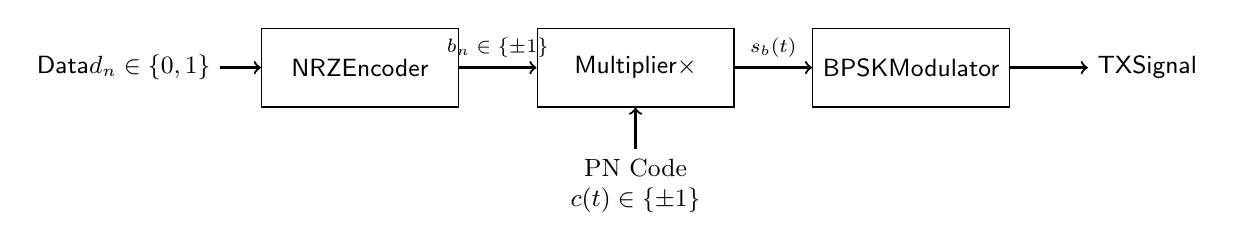
\begin{tikzpicture}[
  block/.style={rectangle, draw, minimum width=2.5cm, minimum height=1cm, font=\sffamily\small},
  node distance=2.5cm,
  font=\small
]
\node (input) {\sffamily Data\\$d_n \in \{0,1\}$};
\node[block, right of=input, node distance=3cm] (nrz) {NRZ\\Encoder};
\node[block, right of=nrz, node distance=3.5cm] (mult) {Multiplier\\$\times$};
\node[block, right of=mult, node distance=3.5cm] (mod) {BPSK\\Modulator};
\node[right of=mod, node distance=3cm] (output) {\sffamily TX\\Signal};

\node[below of=mult, node distance=1.5cm, font=\small, align=center] (code) {PN Code\\$c(t) \in \{\pm 1\}$};

\draw[->,thick] (input) -- (nrz);
\draw[->,thick] (nrz) -- node[above,font=\scriptsize] {$b_n \in \{\pm 1\}$} (mult);
\draw[->,thick] (code) -- (mult);
\draw[->,thick] (mult) -- node[above,font=\scriptsize] {$s_b(t)$} (mod);
\draw[->,thick] (mod) -- (output);
\end{tikzpicture}
\end{center}

\textbf{Mathematical description:}
\begin{equation}
s(t) = A b_n c(t) \cos(2\pi f_c t)
\end{equation}
where:
\begin{itemize}
\item $A$ = carrier amplitude
\item $b_n \in \{\pm 1\}$ = data bit (NRZ encoded)
\item $c(t) \in \{\pm 1\}$ = spreading code (chip sequence)
\item $f_c$ = carrier frequency
\end{itemize}

\textbf{Process:}
\begin{enumerate}
\item \textbf{NRZ encoding:} Map bits to bipolar symbols
  \begin{itemize}
  \item Bit 0 $\rightarrow$ $b_n = +1$
  \item Bit 1 $\rightarrow$ $b_n = -1$
  \end{itemize}
\item \textbf{Spreading:} Multiply data by fast PN code
  \begin{itemize}
  \item Each bit $b_n$ multiplied by $N$ chips: $c_1, c_2, \ldots, c_N$
  \item Result: Wideband chip sequence
  \end{itemize}
\item \textbf{Modulation:} Upconvert to carrier frequency $f_c$
\end{enumerate}

\subsection{Receiver Operation}

The DSSS receiver performs coherent detection with despreading:

\begin{center}
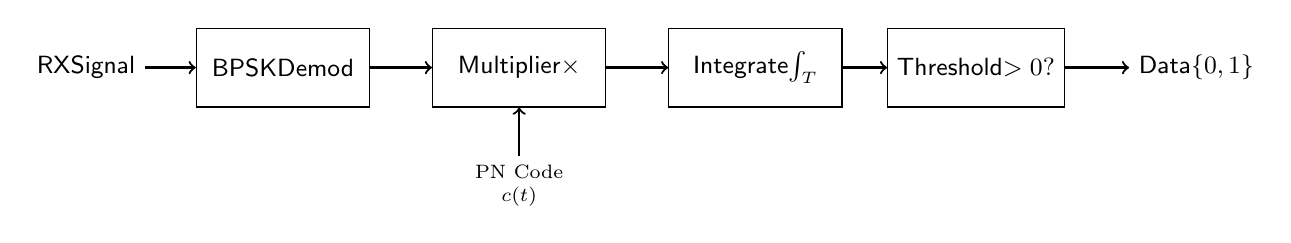
\begin{tikzpicture}[
  block/.style={rectangle, draw, minimum width=2.2cm, minimum height=1cm, font=\sffamily\small},
  node distance=2.2cm,
  font=\small
]
\node (input) {\sffamily RX\\Signal};
\node[block, right of=input, node distance=2.5cm] (demod) {BPSK\\Demod};
\node[block, right of=demod, node distance=3cm] (mult) {Multiplier\\$\times$};
\node[block, right of=mult, node distance=3cm] (int) {Integrate\\$\int_T$};
\node[block, right of=int, node distance=2.8cm] (thresh) {Threshold\\$>0?$};
\node[right of=thresh, node distance=2.8cm] (output) {\sffamily Data\\$\{0,1\}$};

\node[below of=mult, node distance=1.5cm, font=\scriptsize, align=center] (lo) {PN Code\\$c(t)$};

\draw[->,thick] (input) -- (demod);
\draw[->,thick] (demod) -- (mult);
\draw[->,thick] (lo) -- (mult);
\draw[->,thick] (mult) -- (int);
\draw[->,thick] (int) -- (thresh);
\draw[->,thick] (thresh) -- (output);
\end{tikzpicture}
\end{center}

\textbf{Despreading process:}

Received signal (with noise):
\begin{equation}
r(t) = A b_n c(t) \cos(2\pi f_c t) + n(t)
\end{equation}

After demodulation and despreading (multiply by $c(t)$):
\begin{equation}
y(t) = r(t) \cdot c(t) = A b_n c^2(t) + n(t) c(t) = A b_n + n'(t)
\end{equation}

Since $c^2(t) = 1$ (PN code is $\pm 1$), the data is recovered and noise remains spread.

Integration over bit period $T_b$:
\begin{equation}
z = \int_0^{T_b} y(t)\, dt = A b_n T_b + \int_0^{T_b} n'(t)\, dt
\end{equation}

The integrated noise has reduced power by factor $G_p$:
\begin{equation}
\sigma_{n'}^2 = \frac{\sigma_n^2}{G_p}
\end{equation}

\begin{warningbox}
\textbf{Code synchronization is critical.} The receiver PN code must be \textbf{perfectly aligned} with the transmitter code. Phase offset by even one chip destroys correlation and prevents signal recovery. Acquisition can take 1--10 seconds for GPS.
\end{warningbox}

\subsection{Spreading Codes}

\textbf{Requirements for good spreading codes:}
\begin{itemize}
\item \textbf{Pseudorandom:} Appears random but deterministic (reproducible)
\item \textbf{Sharp autocorrelation:} Peak at zero lag, low elsewhere
\item \textbf{Low cross-correlation:} Different codes have low correlation (for CDMA)
\item \textbf{Balance:} Equal number of +1 and $-1$ chips
\end{itemize}

\subsubsection{Maximal-Length Sequences (m-sequences)}

Generated by Linear Feedback Shift Registers (LFSR):

\begin{center}
\begin{tikzpicture}[
  reg/.style={rectangle, draw, minimum width=0.8cm, minimum height=0.8cm, font=\small},
  node distance=1.2cm
]
% Registers
\node[reg] (r1) {$D_1$};
\node[reg, right of=r1] (r2) {$D_2$};
\node[reg, right of=r2] (r3) {$D_3$};
\node[reg, right of=r3] (r4) {$D_4$};
\node[reg, right of=r4] (r5) {$D_5$};
\node[reg, right of=r5] (r6) {$D_6$};
\node[reg, right of=r6] (r7) {$D_7$};

% Output
\node[right of=r7, node distance=1.5cm] (out) {\sffamily Output};
\draw[->,thick] (r7) -- (out);

% Feedback path
\coordinate (tap3) at (r3.south);
\coordinate (tap7) at (r7.south);
\node[circle, draw, inner sep=1pt, font=\scriptsize] (xor) at ($(r1)+(0,-1.2)$) {$\oplus$};

\draw (tap3) -- ++(0,-0.5) -| (xor);
\draw (tap7) -- ++(0,-0.8) -| (xor);
\draw[->,thick] (xor) -| (r1);

\node[below=0.3cm of xor, font=\scriptsize] {Feedback (XOR)};
\node[above=0.3cm of r4, font=\small] {7-stage LFSR (taps: 3, 7)};
\end{tikzpicture}
\end{center}

\textbf{Properties:}
\begin{itemize}
\item Period: $2^n - 1$ (for $n$-stage LFSR)
\item Example: 7-stage LFSR $\rightarrow$ period = 127 chips
\item Good autocorrelation (sharp peak)
\item Poor cross-correlation (not ideal for CDMA)
\end{itemize}

\subsubsection{Gold Codes}

XOR of two m-sequences with specific phase shifts:
\begin{equation}
c_{\mathrm{Gold}}(t) = m_1(t) \oplus m_2(t + \tau)
\end{equation}

\textbf{Properties:}
\begin{itemize}
\item Set of $2^n + 1$ codes (from $n$-stage LFSR)
\item Good autocorrelation \textbf{and} cross-correlation
\item \textbf{Used in GPS:} Each satellite has unique 1023-chip Gold code
\end{itemize}

\begin{calloutbox}[colback=black!5!white,colframe=black]{GPS C/A Code Generation}
GPS uses 1023-chip Gold codes derived from two 10-stage LFSRs:

\textbf{G1 LFSR taps:} [3, 10] (generates $m_1$ sequence)

\textbf{G2 LFSR taps:} [2, 3, 6, 8, 9, 10] (generates $m_2$ sequence)

Each satellite PRN is formed by XORing G1 with phase-shifted G2:
\begin{itemize}
\item PRN 1: G1 $\oplus$ G2[phase $= 5 \oplus 9$]
\item PRN 2: G1 $\oplus$ G2[phase $= 6 \oplus 10$]
\item \ldots (32 satellites total)
\end{itemize}

Period: $2^{10} - 1 = 1023$ chips, repeated every 1~ms.
\end{calloutbox}

\subsubsection{Walsh-Hadamard Codes}

Orthogonal codes with \textbf{zero cross-correlation:}
\begin{equation}
H_1 = [1], \quad H_2 = \begin{bmatrix} 1 & 1 \\ 1 & -1 \end{bmatrix}, \quad H_4 = \begin{bmatrix} 1 & 1 & 1 & 1 \\ 1 & -1 & 1 & -1 \\ 1 & 1 & -1 & -1 \\ 1 & -1 & -1 & 1 \end{bmatrix}
\end{equation}

\textbf{Properties:}
\begin{itemize}
\item Perfectly orthogonal (ideal for CDMA)
\item Length must be power of 2
\item \textbf{Used in IS-95 CDMA:} 64-chip Walsh codes separate users
\end{itemize}

\subsection{CDMA (Code Division Multiple Access)}

CDMA allows multiple users to transmit simultaneously on the same frequency, distinguished by spreading codes.

\begin{center}
\begin{tikzpicture}[
  block/.style={rectangle, draw, minimum width=2cm, minimum height=0.8cm, font=\small},
  node distance=1.2cm
]
% Transmitters
\node[block] (tx1) {User 1\\$d_1 \cdot c_1$};
\node[block, below=0.5cm of tx1] (tx2) {User 2\\$d_2 \cdot c_2$};
\node[block, below=0.5cm of tx2] (tx3) {User 3\\$d_3 \cdot c_3$};
\node[below=0.3cm of tx3, font=\small] (txn) {$\vdots$};

% Summing junction
\node[circle, draw, right=2cm of tx2, minimum size=1cm] (sum) {$\Sigma$};

% Channel
\node[block, right=1.5cm of sum, minimum width=2.5cm] (channel) {Channel\\$+ n(t)$};

% Receiver
\node[block, right=1.5cm of channel, minimum width=2.5cm] (rx) {RX (User 1)\\$\times c_1$, integrate};

% Output
\node[right=1.2cm of rx] (out) {$\hat{d}_1$};

% Connections
\draw[->,thick] (tx1) -| (sum);
\draw[->,thick] (tx2) -- (sum);
\draw[->,thick] (tx3) -| (sum);
\draw[->,thick] (sum) -- (channel);
\draw[->,thick] (channel) -- (rx);
\draw[->,thick] (rx) -- (out);
\end{tikzpicture}
\end{center}

\textbf{Received signal:}
\begin{equation}
r(t) = d_1 c_1(t) + d_2 c_2(t) + d_3 c_3(t) + \cdots + n(t)
\end{equation}

\textbf{User 1 receiver multiplies by $c_1(t)$ and integrates:}
\begin{equation}
\int_T r(t) c_1(t)\, dt = d_1 \underbrace{\int_T c_1^2(t)\, dt}_{=T} + d_2 \underbrace{\int_T c_2(t) c_1(t)\, dt}_{\approx 0} + \cdots + \text{noise}
\end{equation}

Due to low cross-correlation, only User 1's signal integrates to large value; other users appear as noise.

\textbf{CDMA capacity (IS-95):}
\begin{equation}
N_{\mathrm{users}} \approx \frac{G_p}{(E_b/N_0)_{\mathrm{req}}} \cdot (1 + F)^{-1}
\end{equation}
where:
\begin{itemize}
\item $G_p$ = processing gain
\item $(E_b/N_0)_{\mathrm{req}}$ = required SNR for target BER (typically 7~dB)
\item $F$ = frequency reuse factor (0.6--0.85)
\end{itemize}

\begin{calloutbox}{Example: IS-95 CDMA Capacity}
\textbf{Given:}
\begin{itemize}
\item $G_p = 21$ dB (spreading factor 126)
\item $(E_b/N_0)_{\mathrm{req}} = 7$ dB (1\% BER)
\item $F = 0.67$
\end{itemize}

\textbf{Solution:}
$$N_{\mathrm{users}} \approx \frac{126}{5} \times \frac{1}{1.67} \approx 15 \text{ users/sector}$$

With 3 sectors/cell: $\sim$45 users/cell.
\end{calloutbox}

\begin{warningbox}
\textbf{Near-far problem:} In CDMA, users close to the base station overpower distant users. Requires tight \textbf{power control} ($\pm 0.5$ dB accuracy) to maintain equal received power from all users.
\end{warningbox}

\section{Frequency Hopping Spread Spectrum (FHSS)}

FHSS spreads the signal by rapidly switching the carrier frequency according to a pseudorandom pattern.

\subsection{Transmitter Operation}

\begin{center}
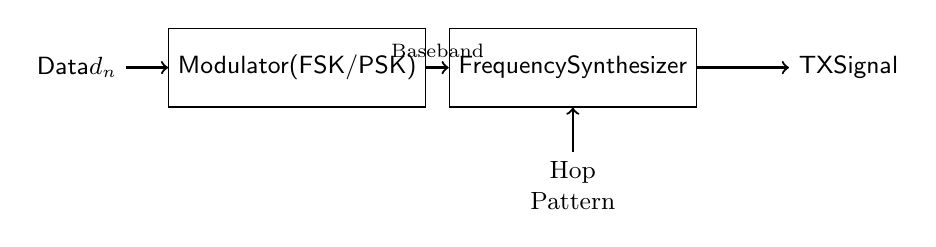
\begin{tikzpicture}[
  block/.style={rectangle, draw, minimum width=2.5cm, minimum height=1cm, font=\sffamily\small},
  node distance=2.5cm,
  font=\small
]
\node (input) {\sffamily Data\\$d_n$};
\node[block, right of=input, node distance=2.8cm] (mod) {Modulator\\(FSK/PSK)};
\node[block, right of=mod, node distance=3.5cm] (mixer) {Frequency\\Synthesizer};
\node[right of=mixer, node distance=3.5cm] (output) {\sffamily TX\\Signal};

\node[below of=mixer, node distance=1.5cm, font=\small, align=center] (hop) {Hop\\Pattern};

\draw[->,thick] (input) -- (mod);
\draw[->,thick] (mod) -- node[above,font=\scriptsize] {Baseband} (mixer);
\draw[->,thick] (hop) -- (mixer);
\draw[->,thick] (mixer) -- (output);
\end{tikzpicture}
\end{center}

\textbf{Time-frequency representation:}

\begin{center}
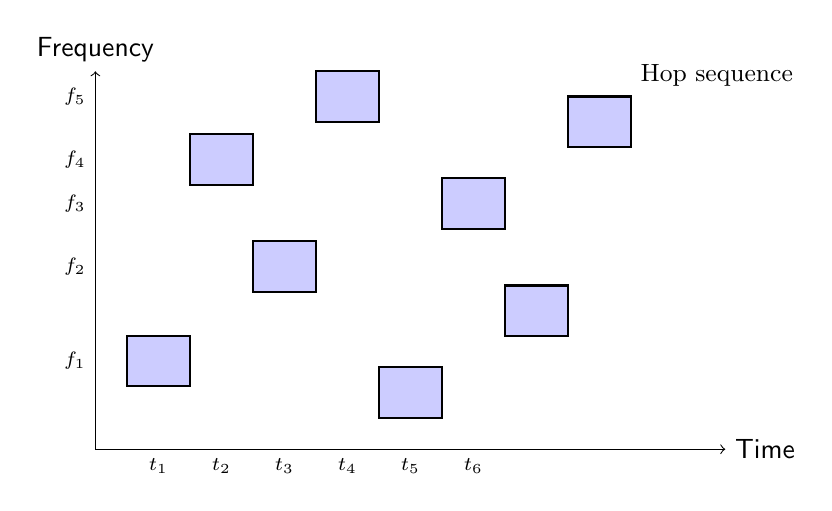
\begin{tikzpicture}[scale=0.8]
\draw[->] (0,0) -- (10,0) node[right] {\sffamily Time};
\draw[->] (0,0) -- (0,6) node[above] {\sffamily Frequency};

% Draw hop pattern
\draw[thick, fill=blue!20] (0.5,1) rectangle (1.5,1.8);
\draw[thick, fill=blue!20] (1.5,4.2) rectangle (2.5,5);
\draw[thick, fill=blue!20] (2.5,2.5) rectangle (3.5,3.3);
\draw[thick, fill=blue!20] (3.5,5.2) rectangle (4.5,6);
\draw[thick, fill=blue!20] (4.5,0.5) rectangle (5.5,1.3);
\draw[thick, fill=blue!20] (5.5,3.5) rectangle (6.5,4.3);
\draw[thick, fill=blue!20] (6.5,1.8) rectangle (7.5,2.6);
\draw[thick, fill=blue!20] (7.5,4.8) rectangle (8.5,5.6);

% Labels
\node[left, font=\scriptsize] at (0,1.4) {$f_1$};
\node[left, font=\scriptsize] at (0,2.9) {$f_2$};
\node[left, font=\scriptsize] at (0,3.9) {$f_3$};
\node[left, font=\scriptsize] at (0,4.6) {$f_4$};
\node[left, font=\scriptsize] at (0,5.6) {$f_5$};

\node[below, font=\scriptsize] at (1,0) {$t_1$};
\node[below, font=\scriptsize] at (2,0) {$t_2$};
\node[below, font=\scriptsize] at (3,0) {$t_3$};
\node[below, font=\scriptsize] at (4,0) {$t_4$};
\node[below, font=\scriptsize] at (5,0) {$t_5$};
\node[below, font=\scriptsize] at (6,0) {$t_6$};

\node[above right, font=\small] at (8.5,5.6) {Hop sequence};
\end{tikzpicture}
\end{center}

\textbf{Key parameters:}
\begin{itemize}
\item \textbf{Hop rate:} Number of hops per second (e.g., 1600 hops/s for Bluetooth)
\item \textbf{Dwell time ($T_h$):} Time spent on each frequency
\item \textbf{Hop set:} Available frequencies $\{f_1, f_2, \ldots, f_M\}$
\item \textbf{Hop sequence:} Pseudorandom pattern $h[n] \in \{1, 2, \ldots, M\}$
\end{itemize}

Processing gain for FHSS:
\begin{equation}
G_p = M = \text{number of hop frequencies}
\end{equation}

or in dB:
\begin{equation}
G_p\,[\mathrm{dB}] = 10\log_{10}(M)
\end{equation}

\subsection{FHSS Variants}

\textbf{1. Fast Frequency Hopping (FFH):}
\begin{itemize}
\item Multiple hops per data symbol
\item Example: Symbol duration = 10~ms, Hop duration = 1~ms $\rightarrow$ 10 hops/symbol
\item \textbf{Advantage:} Diversity against narrowband interference
\end{itemize}

\textbf{2. Slow Frequency Hopping (SFH):}
\begin{itemize}
\item Multiple symbols per hop
\item Example: Hop duration = 10~ms, Symbol duration = 1~ms $\rightarrow$ 10 symbols/hop
\item \textbf{Advantage:} Simpler synchronization
\end{itemize}

\subsection{Receiver Operation}

The FHSS receiver must:
\begin{enumerate}
\item Know the hop pattern (synchronized with transmitter)
\item Track the hop sequence (frequency synthesizer)
\item Demodulate each hop
\end{enumerate}

\textbf{Synchronization requirements:}
\begin{itemize}
\item \textbf{Coarse sync:} Determine which hop in sequence ($\pm 1$ hop)
\item \textbf{Fine sync:} Align within hop duration ($\pm T_h/2$)
\end{itemize}

\begin{calloutbox}{Example: Bluetooth FHSS}
\textbf{Bluetooth Classic (BR/EDR) parameters:}
\begin{itemize}
\item Frequency: 2.4~GHz ISM band
\item Hop set: 79 channels, 1~MHz spacing (2.402--2.480~GHz)
\item Hop rate: 1600 hops/second
\item Dwell time: $T_h = 625~\mu$s
\item Modulation: GFSK (Gaussian FSK)
\item Data rate: 1~Mbps (BR), 2--3~Mbps (EDR)
\end{itemize}

\textbf{Hopping pattern:}
Derived from master device address + clock:
$$h[n] = f(n, \text{BD\_ADDR}, \text{CLK}) \bmod 79$$

\textbf{Adaptive Frequency Hopping (AFH):}
Avoids WiFi-occupied channels by blacklisting them from hop set.
\end{calloutbox}

\subsection{FHSS vs DSSS Comparison}

\begin{center}
\begin{tabular}{@{}lll@{}}
\toprule
\textbf{Aspect} & \textbf{DSSS} & \textbf{FHSS} \\
\midrule
Spreading method & Fast code & Frequency hopping \\
Bandwidth & Continuous wide & Narrow per hop \\
Processing gain & $R_c/R_b$ & $M$ (hop count) \\
Anti-jamming & High (averages) & Moderate (avoids) \\
Multipath & Good (resolves) & Poor (flat fading) \\
Complexity & Correlator & Freq synthesizer \\
Multiple access & CDMA (codes) & FDMA/TDMA \\
Near-far problem & Severe & Minimal \\
Standards & GPS, CDMA & Bluetooth, military \\
\bottomrule
\end{tabular}
\end{center}

\section{Performance Analysis}

\subsection{BER in AWGN Channel}

For DSSS with BPSK modulation in AWGN:
\begin{equation}
\mathrm{BER} = Q\left(\sqrt{\frac{2E_b}{N_0}}\right)
\end{equation}
where:
\begin{itemize}
\item $E_b/N_0$ = energy per bit to noise spectral density ratio
\item $Q(x) = \frac{1}{\sqrt{2\pi}}\int_x^\infty e^{-t^2/2}\, dt$ (Gaussian Q-function)
\end{itemize}

The key is that processing gain allows operation at low SNR:
\begin{equation}
\frac{E_b}{N_0} = \mathrm{SNR} \cdot G_p = \frac{S}{N} \cdot \frac{B_{\mathrm{spread}}}{R_b}
\end{equation}

\begin{calloutbox}{Example: Below-Noise-Floor Reception}
\textbf{Given:}
\begin{itemize}
\item SNR = $-10$ dB (signal 10$\times$ weaker than noise!)
\item Processing gain: $G_p = 30$ dB (GPS-like)
\end{itemize}

\textbf{Solution:}
$$\frac{E_b}{N_0} = -10 + 30 = 20\text{ dB}$$

From BER equation: $\mathrm{BER} = Q(\sqrt{100}) \approx 7.8 \times 10^{-24}$ (excellent!)

This explains how GPS works at $-130$~dBm (20~dB below noise).
\end{calloutbox}

\subsection{Jamming Margin}

The \textbf{jamming margin} determines the maximum jammer power that can be tolerated:
\begin{equation}
M_J = G_p - \left(\frac{J}{S}\right) - \left(\frac{E_b}{N_0}\right)_{\mathrm{req}} - L_{\mathrm{impl}}
\end{equation}
where:
\begin{itemize}
\item $M_J$ = jamming margin (dB)
\item $G_p$ = processing gain (dB)
\item $J/S$ = jammer-to-signal ratio at receiver (dB)
\item $(E_b/N_0)_{\mathrm{req}}$ = required SNR for target BER (dB)
\item $L_{\mathrm{impl}}$ = implementation losses (typically 2--3~dB)
\end{itemize}

\textbf{Positive margin ($M_J > 0$):} Link survives jamming

\textbf{Negative margin ($M_J < 0$):} Link fails

\begin{center}
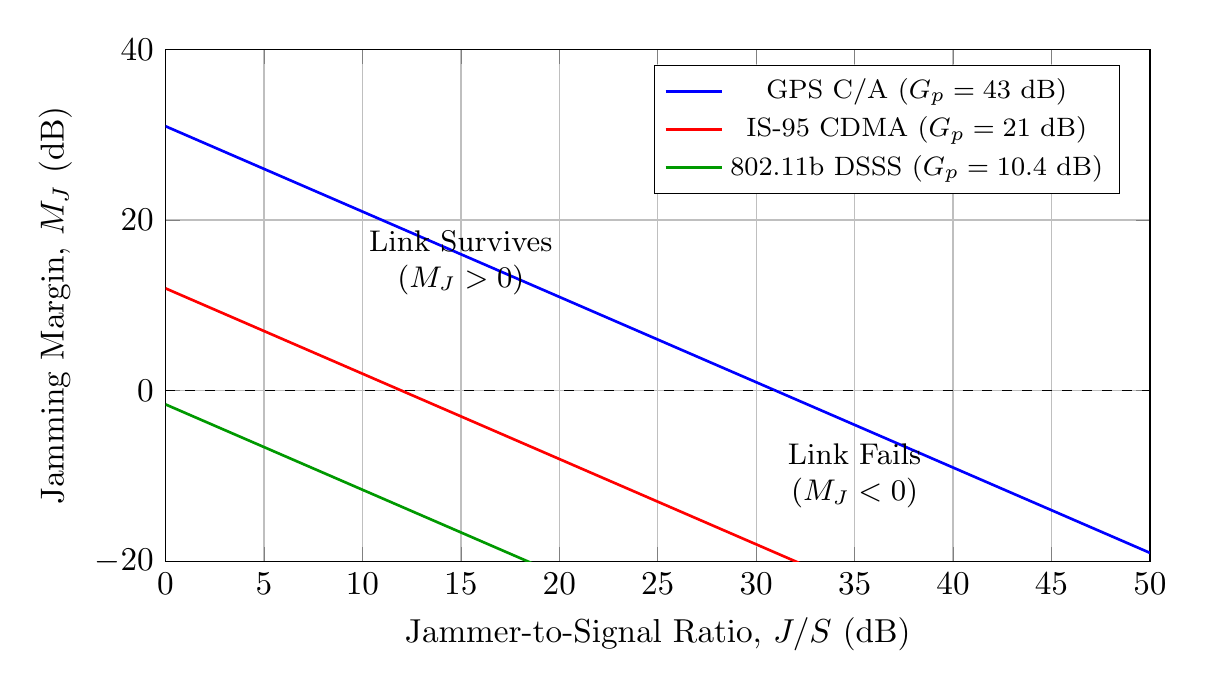
\begin{tikzpicture}[scale=1.2]
\begin{axis}[
  width=12cm,
  height=7cm,
  xlabel={Jammer-to-Signal Ratio, $J/S$ (dB)},
  ylabel={Jamming Margin, $M_J$ (dB)},
  xmin=0, xmax=50,
  ymin=-20, ymax=40,
  grid=major,
  legend pos=north east,
  legend style={font=\footnotesize}
]

% GPS C/A (G_p = 43 dB, (E_b/N_0)_req = 10 dB)
\addplot[blue, thick, domain=0:50] {43 - x - 10 - 2};
\addlegendentry{GPS C/A ($G_p = 43$ dB)}

% IS-95 CDMA (G_p = 21 dB, (E_b/N_0)_req = 7 dB)
\addplot[red, thick, domain=0:50] {21 - x - 7 - 2};
\addlegendentry{IS-95 CDMA ($G_p = 21$ dB)}

% 802.11b DSSS (G_p = 10.4 dB, (E_b/N_0)_req = 10 dB)
\addplot[green!60!black, thick, domain=0:50] {10.4 - x - 10 - 2};
\addlegendentry{802.11b DSSS ($G_p = 10.4$ dB)}

% Zero line
\addplot[black, dashed, domain=0:50] {0};

% Link failure region
\node[align=center, font=\small] at (axis cs:35,-10) {Link Fails\\($M_J < 0$)};
\node[align=center, font=\small] at (axis cs:15,15) {Link Survives\\($M_J > 0$)};
\end{axis}
\end{tikzpicture}
\end{center}

\subsection{Jamming Scenarios}

\textbf{1. Barrage Jamming (wideband noise):}

Jammer spreads power across entire band. Processing gain provides protection:
\begin{equation}
\left(\frac{J}{S}\right)_{\mathrm{despread}} = \left(\frac{J}{S}\right)_{\mathrm{antenna}} - G_p\,[\mathrm{dB}]
\end{equation}

\textbf{2. Partial-Band Jamming:}

Jammer concentrates on fraction $\rho$ of bandwidth:
\begin{itemize}
\item \textbf{DSSS:} Averages jammer over full bandwidth $\rightarrow$ degradation $\propto \rho$
\item \textbf{FHSS:} Hops avoid jammer $(1-\rho)$ fraction of time $\rightarrow$ better performance
\end{itemize}

\textbf{3. Follower Jamming (FHSS target):}

Jammer detects hop and jams that frequency. Countermeasures:
\begin{itemize}
\item Fast hopping (jammer can't track)
\item Adaptive hopping (avoid jammed frequencies)
\end{itemize}

\section{Applications}

\subsection{GPS (Global Positioning System)}

\textbf{Architecture:}
\begin{itemize}
\item 31 satellites in MEO (20,200~km altitude)
\item Each transmits unique Gold code (PRN 1--32)
\item Carrier: L1 = 1575.42~MHz, L2 = 1227.60~MHz
\end{itemize}

\textbf{C/A Code (Civilian):}
\begin{itemize}
\item Modulation: BPSK
\item Chip rate: 1.023~Mcps
\item Code length: 1023 chips (1~ms period)
\item Data rate: 50~bps (navigation message)
\item Processing gain: 43~dB
\end{itemize}

\textbf{Link budget:}
\begin{itemize}
\item TX power: 27~W (44~dBm)
\item TX antenna gain: 13~dBi (toward Earth)
\item Free-space path loss (20,200~km @ 1.5~GHz): 184~dB
\item RX antenna gain: 3~dBi (patch antenna)
\item Received power: $44 + 13 - 184 + 3 = -124$~dBm
\item Noise floor ($B = 2$~MHz): $-114$~dBm
\item SNR: $-124 - (-114) = -10$~dB (below noise!)
\item After despreading: $-10 + 43 = 33$~dB (excellent SNR)
\end{itemize}

\textbf{M-Code (Military):}
\begin{itemize}
\item Chip rate: 5.115~Mcps (5$\times$ faster than C/A)
\item Processing gain: $\sim$50~dB
\item Modulation: BOC(10,5) --- Binary Offset Carrier
\item Security: Encrypted, authenticated (NSA keys)
\item Anti-jam margin: 60~dB (tolerates strong jamming)
\end{itemize}

\subsection{Bluetooth}

\textbf{Bluetooth Classic (BR/EDR):}
\begin{itemize}
\item Frequency: 2.4~GHz ISM band
\item Hop set: 79 channels (1~MHz spacing)
\item Hop rate: 1600 hops/second
\item Modulation: GFSK (Gaussian FSK)
\item Data rate: 1--3~Mbps
\item Range: 10~m (Class 2), 100~m (Class 1)
\end{itemize}

\textbf{Network topology:}
\begin{itemize}
\item \textbf{Piconet:} Master + up to 7 slaves
\item \textbf{Scatternet:} Overlapping piconets
\item Each piconet: Unique hopping pattern
\end{itemize}

\textbf{Adaptive Frequency Hopping (AFH):}

Avoids WiFi-occupied channels:
\begin{enumerate}
\item Monitor channel quality (BER, RSSI)
\item Blacklist poor channels (typically 20--30 channels)
\item Hop only among good channels (49--59 channels)
\item Update blacklist periodically
\end{enumerate}

\subsection{IEEE 802.11b WiFi (Legacy DSSS)}

\textbf{Parameters:}
\begin{itemize}
\item Frequency: 2.4~GHz ISM band
\item Chip rate: 11~Mcps
\item Data rate: 1--11~Mbps
\item Spreading: 11-chip Barker sequence (1--2~Mbps)
\item CCK codes (5.5, 11~Mbps)
\item Processing gain: 10.4~dB (1~Mbps mode)
\end{itemize}

\textbf{11-chip Barker code:}
$$[+1, -1, +1, +1, -1, +1, +1, +1, -1, -1, -1]$$

\textbf{Properties:}
\begin{itemize}
\item Autocorrelation: Peak = 11, sidelobes = 1 (excellent!)
\item Provides interference rejection
\end{itemize}

\textbf{Obsolescence:} Replaced by OFDM in 802.11g (2003) for higher spectral efficiency.

\subsection{IS-95 CDMA Cellular}

\textbf{Architecture:}
\begin{itemize}
\item Frequency: 800~MHz, 1900~MHz (US)
\item Bandwidth: 1.25~MHz per carrier
\item Chip rate: 1.2288~Mcps
\item Spreading factor: 64--256 (variable rate)
\item Walsh codes: 64 orthogonal channels
\end{itemize}

\textbf{Capacity:}
\begin{itemize}
\item Processing gain: 21~dB (SF = 128)
\item Users/sector: 15--20 (voice)
\item Soft handoff: Multiple cells serve one user
\end{itemize}

\textbf{Power control:}
\begin{itemize}
\item Rate: 800~Hz (every 1.25~ms)
\item Accuracy: $\pm 0.5$~dB
\item Range: 80~dB (to combat near-far problem)
\end{itemize}

\textbf{Status:} Retired in US (Verizon, Sprint) around 2020, replaced by LTE/5G.

\subsection{Military Link 16 (JTIDS)}

\textbf{Purpose:} NATO/US tactical data link for coordinated operations.

\textbf{Parameters:}
\begin{itemize}
\item Frequency: 960--1215~MHz (L-band)
\item Modulation: MSK (Minimum Shift Keying)
\item Waveform: 51 frequency channels
\item Hop rate: 70,000 hops/second ($\sim$14~$\mu$s per hop)
\item Security: Time-varying encryption (TRANSEC)
\item Data rate: 31.6--115.2~kbps
\end{itemize}

\textbf{Network:}
\begin{itemize}
\item TDMA: 128 time slots per 12~seconds
\item Nodes: Aircraft, ships, ground stations
\item Collision-free multiple access
\end{itemize}

\textbf{TRANSEC (Transmission Security):}
\begin{itemize}
\item Hopping pattern: Cryptographically secured
\item Changes every 12~seconds (epoch)
\item Synchronized via GPS time
\item Enemy cannot predict next hop
\end{itemize}

\textbf{Result:}
\begin{itemize}
\item LPI/LPD: Signal appears as brief noise burst
\item AJ: Hops faster than jammer can follow
\item Covertness: No fixed frequency to monitor
\end{itemize}

\section{Worked Example: GPS Link Budget with Jamming}

\textbf{Problem:} A GPS receiver experiences jamming. Determine if the link survives.

\subsection*{Given}

\textbf{GPS parameters:}
\begin{itemize}
\item Received signal power: $P_s = -130$~dBm
\item Processing gain: $G_p = 43$~dB (C/A code)
\item Required $(E_b/N_0)_{\mathrm{req}} = 10$~dB (for BER $= 10^{-6}$)
\item Implementation losses: $L_{\mathrm{impl}} = 2$~dB
\end{itemize}

\textbf{Jammer:}
\begin{itemize}
\item Jammer power at receiver: $P_J = -90$~dBm (barrage noise)
\end{itemize}

\textbf{Noise:}
\begin{itemize}
\item Thermal noise: $N_0 = -174$~dBm/Hz
\item Bandwidth: $B = 2$~MHz = 63~dBHz
\item Noise power: $N = N_0 + 10\log_{10}(B) = -174 + 63 = -111$~dBm
\end{itemize}

\subsection*{Solution}

\textbf{Step 1: Calculate J/S ratio}
\begin{equation}
\frac{J}{S} = P_J - P_s = -90 - (-130) = 40\text{ dB}
\end{equation}

The jammer is 10,000$\times$ stronger than the GPS signal!

\textbf{Step 2: Calculate jamming margin}
\begin{equation}
M_J = G_p - \frac{J}{S} - \left(\frac{E_b}{N_0}\right)_{\mathrm{req}} - L_{\mathrm{impl}}
\end{equation}
\begin{equation}
M_J = 43 - 40 - 10 - 2 = -9\text{ dB}
\end{equation}

\textbf{Result:} Negative margin $\rightarrow$ \textbf{Link fails!}

\textbf{Step 3: Mitigation --- Directional antenna}

Use directional antenna with:
\begin{itemize}
\item Gain toward satellites: $+20$~dBi
\item Null toward jammer (ground-based): $-20$~dB attenuation
\end{itemize}

Effective J/S after antenna:
\begin{equation}
\left(\frac{J}{S}\right)_{\mathrm{eff}} = 40 - 20 - 20 = 0\text{ dB}
\end{equation}

New jamming margin:
\begin{equation}
M_J = 43 - 0 - 10 - 2 = 31\text{ dB}
\end{equation}

\textbf{Result:} \textbf{Link survives} with 31~dB margin!

\begin{calloutbox}[colback=black!8!white,colframe=black]{Summary}
\textbf{Without directional antenna:} Jammer overpowers GPS by 9~dB $\rightarrow$ Link fails

\textbf{With directional antenna:} 40~dB total suppression (20~dB gain + 20~dB null) $\rightarrow$ Link survives with comfortable margin

\textbf{Lesson:} Spread spectrum alone is insufficient against strong jamming. Spatial filtering (directional antennas, adaptive arrays) is essential for military GPS receivers.
\end{calloutbox}

\section{Advantages and Disadvantages}

\subsection*{Advantages}

\begin{enumerate}
\item \textbf{Anti-jamming:} Processing gain overcomes interference
\item \textbf{LPI/LPD:} Signal hidden in noise (military stealth)
\item \textbf{Below-noise-floor operation:} GPS works at SNR $= -10$~dB
\item \textbf{Multiple access:} CDMA allows many users simultaneously
\item \textbf{Multipath resistance (DSSS):} Wideband signals resolve path delays
\item \textbf{Privacy:} Eavesdropping requires spreading code
\item \textbf{Coexistence:} Graceful degradation with other systems
\end{enumerate}

\subsection*{Disadvantages}

\begin{enumerate}
\item \textbf{Bandwidth inefficient:} Uses 100--1000$\times$ more spectrum than narrowband
\item \textbf{Complex synchronization:} Code/frequency alignment required (acquisition time 1--10~s)
\item \textbf{Near-far problem (DSSS CDMA):} Strong users drown weak ones $\rightarrow$ tight power control needed
\item \textbf{Processing overhead:} Correlators, frequency synthesizers (high power consumption)
\item \textbf{Acquisition time:} GPS cold start can take 30--60~seconds
\end{enumerate}

\section{Summary}

\begin{center}
\begin{tabular}{@{}lll@{}}
\toprule
\textbf{Parameter} & \textbf{DSSS} & \textbf{FHSS} \\
\midrule
Spreading method & Fast PN code & Frequency hopping \\
Processing gain & $R_c/R_b$ & $M$ (hop count) \\
Bandwidth & Continuous wide & Narrow per hop \\
Anti-jamming & Excellent & Good \\
Multipath resistance & Good & Poor \\
Synchronization & Code alignment & Hop tracking \\
Complexity & Correlator & Freq synthesizer \\
Multiple access & CDMA & FDMA/TDMA \\
Examples & GPS, CDMA & Bluetooth, military \\
\bottomrule
\end{tabular}
\end{center}

\textbf{Key equations:}
\begin{itemize}
\item Processing gain: $G_p = B_{\mathrm{spread}}/B_{\mathrm{info}} = R_c/R_b$
\item SNR improvement: $\mathrm{SNR}_{\mathrm{out}} = \mathrm{SNR}_{\mathrm{in}} + G_p$
\item Jamming margin: $M_J = G_p - J/S - (E_b/N_0)_{\mathrm{req}} - L_{\mathrm{impl}}$
\end{itemize}

\section{Further Reading}

\begin{itemize}
\item \textbf{Chapter 2:} Binary Phase-Shift Keying (BPSK)---underlying modulation for DSSS
\item \textbf{Chapter 6:} Frequency-Shift Keying (FSK)---modulation for FHSS
\item \textbf{Chapter 12:} Constellation Diagrams---visualization of spread signals
\item \textbf{Chapter 18:} Bit Error Rate Analysis---BER performance with processing gain
\item \textbf{Chapter 20:} Shannon's Channel Capacity Theorem---theoretical foundation
\item \textbf{Chapter 22:} Forward Error Correction---coding with spread spectrum
\item \textbf{Chapter 25:} Synchronization---code acquisition and tracking
\item \textbf{Chapter 28:} Military \& Covert Communications---LPI/LPD systems, GPS M-code
\item \textbf{Chapter 35:} Real-World System Examples---GPS, Bluetooth, WiFi, Link 16
\end{itemize}
